\begin{frame}
  \frametitle{\problemtitle}

  \begin{itemize}
  \item Given is a $n\times n$ grid of dance tiles ($3\leq n\leq 500$).
  \item The dance alternates moves similar to a knight in chess.
    \begin{itemize}
  \item The first move $(a,b)$ goes $a$ along one axis and $b$ along the other axis.
  \item The second move $(c,d)$ goes $c$ along one axis and $d$ along the other axis.
    \end{itemize}
  \item You start in the top left corner with either of the two moves.
  \item How many tiles can you reach during \emph{some} performance of the dance?
  \end{itemize}

  \centering
  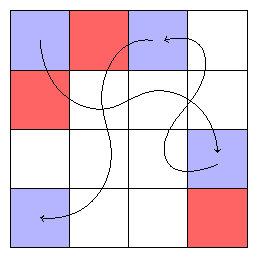
\includegraphics[width=0.22\textwidth]{figure} \\
  \small
  Illustration of Sample Input 3, showing a dance that begins in the top left corner of a $4\times 4$ grid and ends in the bottom left corner, visiting the blue squares along the way.
  There are $13$ reachable squares in total.
  The three squares highlighted in red cannot be part of any dance performance.

\end{frame}
